\chapter{HASIL DAN PEMBAHASAN}
\label{chap:hasilpembahasan}

Pada bab ini dipaparkan hasil dari eksperimen yang dilakukan pada penelitian ini.
Hasil dari training berupa \emph{mean episode rewards} dari agen \emph{attacker} dan agen \emph{defender},
waktu training, rerata waktu inferensi, rerata waktu proses \emph{actions}, rerata waktu \emph{environment} menunggu,
rerata waktu pemrosesan observasi mentah, dan presentase penggunaan CPU serta RAM.

Hasil dari evaluasi berupa performa algoritma jika dilawankan dengan generasi sebelum dan sesudahnya,
serta evaluasi performa algoritma dalam skenario \emph{environment} yang berbeda berupa area lebih besar
(16x16).

\section{Hasil Training}

Dalam eksperimen RL, hal yang paling penting untuk diperhatikan adalah nilai \emph{rewards} (\emph{episode rewards}) yang didapatkan oleh agen
selama training. Performa agen RL dapat diukur dengan seberapa banyak reward yang telah didapatkan oleh agen.
Dari eksperimen yang telah dilakukan, didapatkan beberapa nilai \emph{rewards}, 
seperti \emph{mean episode rewards}, \emph{max episode rewards}, dan \emph{min episode rewards} untuk kedua agen dengan keempat algoritma yang diuji coba.
\emph{Mean episode rewards} merupakan rerata nilai \emph{rewards} yang didapatkan oleh agen selama satu episode.

Nilai \emph{mean episode rewards} menunjukan akan performa kedua agen saat training.
Agen \emph{attacker} yang berhasil mencapai nilai \emph{atttacker mean episode reward} sebesar 20 poin atau ke atas
merupakan agen attacker yang dapat secara konsisten menyelesaikan tujuannya, yaitu menghancurkan kota.
Hal ini karena \emph{reward} yang didapatkan oleh agen \emph{attacker} dalam menghancurkan kota adalah 20 poin.

Nilai \emph{max episode rewards} merupakan nilai tertinggi yang didapatkan oleh agen selama training berlangsung.
Sebaliknya, nilai \emph{min episode rewards} merupakan nilai terendah yang didapatkan oleh agen selama training.


\begin{table}[h]
  \centering
  \label{table:meanEpisodeReward}
  \caption{Tabel nilai akhir \emph{mean episode rewards} kedua agen}
  \begin{tabular}{|c|c|c|}
  \hline
  \textbf{Algorithm} & \textbf{\begin{tabular}[c]{@{}c@{}}Attacker Mean\\ Episode Reward\end{tabular}} & \textbf{\begin{tabular}[c]{@{}c@{}}Defender Mean\\ Episode Reward\end{tabular}} \\ \hline
  APE-X DQN           & 20.62                                                                           & 2.36                                                                            \\ \hline
  DQN                & 2.05                                                                            & 0.71                                                                            \\ \hline
  PPO                & -3.2                                                                            & -1.9                                                                            \\ \hline
  IMPALA             & 1.041                                                                           & 2.24                                                                            \\ \hline
  \end{tabular}
\end{table}

\subsection{Attacker Mean Episode Rewards}

\begin{figure}[H]
  \centering
    % Nama dari file gambar yang diinputkan
    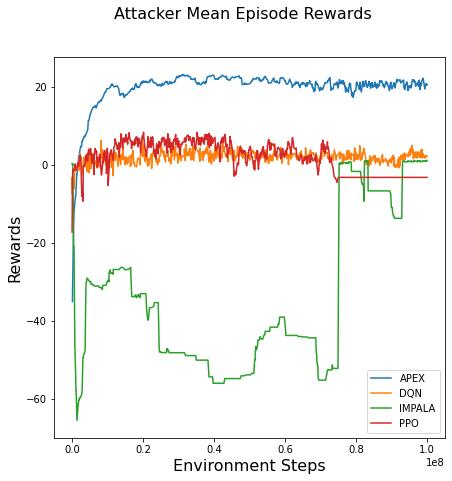
\includegraphics[scale=0.9]{gambar/attacker_reward_mean.jpg}
    % Keterangan gambar yang diinputkan
    \caption{Grafik menunjukan \emph{mean episode rewards} dari agen \emph{attacker}.
    Biru: APE-X DQN, oranye: DQN, hijau: IMPALA, merah: PPO}
    % Label referensi dari gambar yang diinputkan
    \label{fig:attackerMeanEpisodeGraph}
\end{figure}

Dari grafik \ref{fig:attackerMeanEpisodeGraph}, APE-X DQN merupakan algoritma yang paling baik,
jauh di atas algoritma lain. APE-X DQN mencapai nilai 20 poin sekitar pada 1.5 \emph{environment steps}.
APE-X DQN berkonvergensi di sekitar nilai 20 poin ini sebelum 2 juta \emph{environment steps}.
Mengingat 20 poin merupakan nilai \emph{reward} ketika agen \emph{attacker} menghancurkan kota,
agen \emph{attacker} APE-X DQN secara konsisten telah menyelesaikan tujuan tersebut.

Algoritma lain jauh dibawah performa APE-X DQN. Algoritma DQN selalu di bawah 5 poin dan tidak meningkat secara signifikan.
Algoritma PPO mencapai nilai 5 poin pada sekitar 1.5 juta \emph{environment steps}, akan tetapi menurun setelah 5 juta
\emph{environment steps}. PPO juga mengalami \emph{flatline} dimana secara tiba tiba algoritma tersebut
tidak mengalami peningkatan atau penurunan nilai \emph{rewards} pada sebelum 8 juta \emph{environment steps}
sampai akhir sesi. PPO merupakan algoritma terburuk pada grafik ini. IMPALA merupakan algoritma yang paling tidak stabil pada grafik ini.
Nilai \emph{mean episode rewards} agen \emph{attacker} IMPALA selalu di bawah -20 poin sampai
sekitar sebelum 8 juta \emph{environment steps} dimana IMPALA melonjak ke nilai 0 poin.
Nilai poin negatif dari IMPALA hanya bisa dicapai jika \emph{unit} agen \emph{attacker} mencoba untuk keluar
dari batas \emph{environment} secara terus menerus.

\subsection{Defender Mean Episode Rewards}

\begin{figure}[H]
  \centering
    % Nama dari file gambar yang diinputkan
    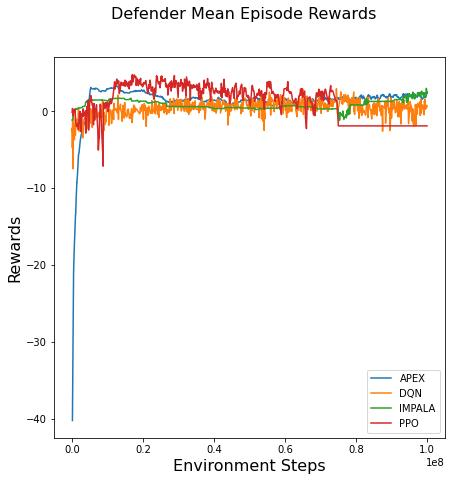
\includegraphics[scale=0.9]{gambar/defender_reward_mean.jpg}
    % Keterangan gambar yang diinputkan
    \caption{Grafik menunjukan \emph{mean episode rewards} dari agen \emph{defender}.
    Biru: APE-X DQN, oranye: DQN, hijau: IMPALA, merah: PPO}
    % Label referensi dari gambar yang diinputkan
    \label{fig:defenderMeanEpisodeGraph}
\end{figure}

Perubahan nilai \emph{rewards} algoritma dalam grafik \ref{fig:defenderMeanEpisodeGraph} jauh lebih stabil.
Hal ini disebabkan karena nilai \emph{general reward} yang diterima oleh agen \emph{defender} tidak memiliki varian yang tinggi,
dibandingkan dengan agen \emph{attacker} yang memerima 20 poin ketika menghancurkan kota.

APE-X DQN memulai dengan -40 poin akan tetapi secara cepat melonjak ke atas 2 poin.
Sama dengan di grafik \ref{fig:attackerMeanEpisodeGraph}, APE-X DQN merupakan algoritma paling stabil.
APE-X DQN juga salah satu algoritma dengan performa terbaik, bersebelahan dengan IMPALA.

DQN tidak berhasil melakukan konvergensi dengan baik dan nilainya tidak stabil sampai akhir sesi.
PPO juga merupakan algoritma terburuk pada grafik ini. Keadaan \emph{flatline} sama yang dialami PPO pada grafik
\ref{fig:attackerMeanEpisodeGraph} juga dapat dilihat disini.

\subsection{Attacker Min dan Max Episode Rewards}
\begin{table}[H]
  \centering
  \caption{Tabel nilai min dan max \emph{episode rewards} agen \emph{attacker}}
  \label{table:attackerMinMaxRewards}
  \begin{tabular}{|c|c|c|}
  \hline
  \textbf{Algorithm} & \textbf{\begin{tabular}[c]{@{}c@{}}Attacker Min\\ Episode Reward\end{tabular}} & \textbf{\begin{tabular}[c]{@{}c@{}}Attacker Max\\ Episode Reward\end{tabular}} \\ \hline
  APE-X DQN           & -0.9                                                                           & 30                                                                             \\ \hline
  DQN                & -15.4                                                                          & 25.2                                                                           \\ \hline
  PPO                & 0                                                                              & 2.8                                                                            \\ \hline
  IMPALA             & -26.2                                                                          & 14                                                                             \\ \hline
  \end{tabular}
\end{table}

Dari nilai \emph{max episode rewards} APE-X DQN merupakan algoritma tertinggi paka 30 poin.
Diikuti oleh DQN pada 25.2 poin.
Kedua algoritma ini berada di atas 20 poin, yang berarti bahwa agen \emph{attacker} pada algoritma tersebut
berhasil menghancurkan kota dalam salah satu episodenya.
30 poin pada APE-X DQN menunjukan bahwa APE-X DQN dapat menghancurkan kota dan sekaligus membunuh seluruh unit agen
defender pada salah satu episodenya.
30 poin merupakan poin yang hampir paling tinggi untuk bisa dicapai.
IMPALA mendapatkan 14 poin, yang berarti agen \emph{attacker} algoritma ini dapat menghancurkan kota dalam salah satu episodenya,
namun melakukannya dengan giliran yang lebih banyak dibandingkan DQN atau APE-X DQN.
PPO memiliki nilai max hanya sebesar 2.8 menunjukan bahwa agen \emph{attacker} PPO berhasil menghancurkan kota namun memerlukan hampir seluruh giliran yang ada.

Nilai \emph{min episode rewards} menunjukan performa terburuk agen \emph{attacker} pada salah satu episode.
PPO merupakan algoritma yang memiliki nilai minimum tertinggi sebesar 0.
Jika dibandingkan dengan nilai maksimum milik PPO, PPO merupakan algoritma yang cukup stabil karena perbedaan antara
minimum dan maksimum sangat kecil.
APE-X DQN merupakan algoritma kedua terbaik denga minimum sebesar -0.9, diikuti oleh DQN pada -15.4 dan IMPALA -26.2.

\subsection{Defender Min dan Max Episode Rewards}

\begin{table}[H]
  \centering
  \caption{Tabel nilai min dan max \emph{episode rewards} agen \emph{defender}}
  \label{table:defenderMinMaxRewards}
  \begin{tabular}{|c|c|c|}
  \hline
  \textbf{Algorithm} & \textbf{\begin{tabular}[c]{@{}c@{}}Defender Min\\ Episode Reward\end{tabular}} & \textbf{\begin{tabular}[c]{@{}c@{}}Defender Max\\ Episode Reward\end{tabular}} \\ \hline
  APE-X DQN           & 0                                                                              & 9.2                                                                            \\ \hline
  DQN                & -11.8                                                                          & 10.7                                                                           \\ \hline
  PPO                & -24.2                                                                          & 7.5                                                                            \\ \hline
  IMPALA             & -2.2                                                                           & 8.6                                                                            \\ \hline
  \end{tabular}
\end{table}

Pada nilai \emph{max episode rewards} agen \emph{defender}, seluruh algoritma memiliki nilai yang tidak jauh berbeda antara satu sama lain.
DQN menungguli algoritma lain pada nilai 10l7, diikuti oleh APE-X DQN pada 9.2, IMPALA 8.6 dan terakhir PPO pada 7.5.
Agen \emph{defender} seluruh algoritma dapat membunuh beberapa atau seluruh unit milik agen \emph{attacker} pada salah satu episodenya.
Maka performa terbaik dari seluruh algoritma hampir sama antar satu sama lain.

Pada nilai \emph{min episode rewards} agen \emph{defender}, APE-X DQN merupakan algoritma dengan nilai minimum tertinggi.
Nilai 0 yang didapatkan merupakan keadaan dimana agen \emph{defender} tidak melakukan banyak kesalahan pergerakan (bergerak ke ujung area)
atau dapat mengkompensasi kesalahan tersebut dengan membunuh beberapa unit lawan.
Berbalik dengan agen \emph{attacker}, IMPALA merupakan algoritma yang paling stabil dalam perbedaan nilai minimum dan maksimum.
Sedangkan PPO tidak sestabil nilai maksimum dan minimum agen \emph{attacker}.
PPO merupakan algoritma dengan nilai minimum terendah.

\subsection{Waktu dan Pemakaian Resource Algoritma}

\begin{table}[H]
  \centering
  \caption{Training, Inference, Processing Time, and Resource Usage}
  \label{table:timeAndResourceSpent}
  \begin{tabular}{|l|l|l|l|l|}
      \hline
      \textbf{Metrics}                                                            & \textbf{APE-X DQN} & \textbf{DQN}     & \textbf{PPO}     & \textbf{IMPALA}  \\ \hline
      \begin{tabular}[c]{@{}l@{}}Total Training \\ Time\end{tabular}          & 1d 17h             & 8d 7h            & 3d 3h             & 23h     \\ \hline
      \begin{tabular}[c]{@{}l@{}}Mean Inference \\ (ms)\end{tabular}          & 3.406     & 9.191   & 2.446   & 1.862   \\ \hline
      \begin{tabular}[c]{@{}l@{}}Mean Action \\ Processing (ms)\end{tabular}  & 0.06758   & 0.07171 & 0.05702 & 0.05636 \\ \hline
      \begin{tabular}[c]{@{}l@{}}Mean Environment \\ Wait (ms)\end{tabular}   & 0.457     & 0.4237  & 0.414   & 0.4119  \\ \hline
      \begin{tabular}[c]{@{}l@{}}Mean Raw Obs \\ Processing (ms)\end{tabular} & 0.3512    & 0.2834  & 0.2363  & 0.2143  \\ \hline
      RAM Utilization                                                         & 82.3\%    & 38.82\% & 36.1\%  & 33.2\%  \\ \hline
      CPU Utilization                                                         & 79.95\%   & 40.78\% & 39.63\% & 63.51\% \\ \hline
  \end{tabular}
\end{table}

Tabel \ref{table:timeAndResourceSpent} menunjukan bahwa IMPALA merupakan algoritma tercepat
untuk menyelesaikan 10 juta \emph{environment step} dengan \emph{total training time} selama
23 jam. APE-X DQN mengikuti IMPALA tidak jauh setelahnya dengan \emph{total training time}
selama 1 hari 7 jam (30 jam). PPO memerlukan waktu lebih dari 3x lebih lama dengan \emph{total training time}
sebesar 3 hari 3 jam (75 jam). DQN merupakan algoritma terlama yang memerlukan 8 hari 7 jam (199 jam).

IMPALA juga merupakan algoritma tercepat dalam inferensi dengan nilai \emph{mean inference} sebesar
1.862 ms. PPO merupakan algoritma tercepat kedua dengan \emph{mean inference} sebesar 2.446 ms walaupun \emph{total
training time} PPO lebih lambat dari APE-X DQN, APE-X DQN berada di setelah PPO dengan \emph{mean inference}
sebesar 3.406 ms. DQN merupakan algoritma terlama dalam melakukan inferensi dengan 9.191 ms.
\emph{Metrics} lainnya seperti \emph{mean action processing}, \emph{mean environment wait}, dan \emph{mean raw obs processing}
tidak berbeda jauh antara satu algoritma dengan algoritma lainnya.

Pada penggunaan RAM dan CPU, APE-X DQN merupakan algoritma yang menggunakan CPU dan RAM terbanyak
dengan penggunaan CPU sebesar 79.95\% dan RAM sebesar 82.3\%. Hal ini disebabkan oleh penggunaan CPU
APE-X DQN yang menggunakan seluruh 8 \emph{cores} dibandingkan algoritma lain yang menggunakan 4 \emph{cores}
dengan jumlah \emph{workers} yang sama (3 \emph{workers}). IMPALA merupakan algoritma DRL
terdistribusi lainnya yang menggunakan CPU terbanyak setelah APE-X DQN dengan penggunaan sebesar
63.51\%. Akan tetapi penggunaan RAM dari IMPALA jauh lebih minim dengan penggunaan sebesar 33.2\%.
PPO dan DQN menggunakan CPU dan RAM sama banyaknya dengan penggunaan CPU sebesar 39-40\% dan RAM
sebesar 36-39\%.

\section{Hasil Evaluasi}
Setelah dilakukan \emph{training}, terdapat dua macam evaluasi yang dilakukan.
Evaluasi antar generasi algoritma dan evaluasi dengan \emph{environment} yang lebih luas.
Hasil dari kedua evaluasi merupakan \emph{rewards} yang didapatkan oleh agen pada setiap generasi algoritma.
Evaluasi dimulai dari generasi 1 agen \emph{attakcer} melawan seluruh generasi dari agen \emph{defender}.
Kemudian dilanjut pada generasi 2 agen \emph{attacker} melawan seluruh generasi dari agen \emph{defender}.
Hingga seluruh generasi dari sebuah algoritma sudah melawan satu sama lain.

\subsection{Hasil Evaluasi Antar Generasi Algoritma}

\begin{table}[H]
  \centering
  \caption{Evaluasi Antar Generasi DQN}
  \label{table:dqnVersusResult}
  \begin{tabular}{|c|c|c|c|}
  \hline
  \textbf{\begin{tabular}[c]{@{}c@{}}Attacker Agent\\ Generation\end{tabular}} & \textbf{\begin{tabular}[c]{@{}c@{}}Defender Agent\\ Generation\end{tabular}} & \textbf{\begin{tabular}[c]{@{}c@{}}Attacker Mean\\ Episode Rewards\end{tabular}} & \textbf{\begin{tabular}[c]{@{}c@{}}Defender Mean\\ Episode Rewards\end{tabular}} \\ \hline
  \multirow{4}{*}{1}                                                           & 1                                                                            & -80.15                                                                           & -6.53                                                                            \\ \cline{2-4} 
                                                                               & 2                                                                            & -71.4                                                                            & -15.75                                                                           \\ \cline{2-4} 
                                                                               & 3                                                                            & -79.617                                                                          & -53.08                                                                           \\ \cline{2-4} 
                                                                               & 4                                                                            & -82.76                                                                           & -37.38                                                                           \\ \hline
  \multirow{4}{*}{2}                                                           & 1                                                                            & -0.46                                                                            & -18.46                                                                           \\ \cline{2-4} 
                                                                               & 2                                                                            & -0.56                                                                            & -13.53                                                                           \\ \cline{2-4} 
                                                                               & 3                                                                            & -0.41                                                                            & -48.12                                                                           \\ \cline{2-4} 
                                                                               & 4                                                                            & -0.66                                                                            & -27.16                                                                           \\ \hline
  \multirow{4}{*}{3}                                                           & 1                                                                            & -0.72                                                                            & -16.53                                                                           \\ \cline{2-4} 
                                                                               & 2                                                                            & -1.98                                                                            & -13.38                                                                           \\ \cline{2-4} 
                                                                               & 3                                                                            & -1.68                                                                            & -46.59                                                                           \\ \cline{2-4} 
                                                                               & 4                                                                            & -2.6                                                                             & -25.1                                                                            \\ \hline
  \multirow{4}{*}{4}                                                           & 1                                                                            & -0.71                                                                            & -15.78                                                                           \\ \cline{2-4} 
                                                                               & 2                                                                            & -0.65                                                                            & -11.86                                                                           \\ \cline{2-4} 
                                                                               & 3                                                                            & -1.30                                                                            & -48.36                                                                           \\ \cline{2-4} 
                                                                               & 4                                                                            & -0.52                                                                            & -28.56                                                                           \\ \hline
  \end{tabular}
\end{table}

Pada algoritma DQN, performa antar generasi agen \emph{attacker} memmiliki nilai \emph{mean episode rewards} yang mirip, kecuali generasi pertama.
Performa agen \emph{attacker} generasi 1 jauh dibawah performa generasi-generasi selanjutnya.
Ini merupakan salah satu dampak penggunaan \emph{epsilon greedy} dalam algoritma DQN.
Algoritma DQN akan melakukan aksi secara acak pada saat \emph{training} untuk melakukan eksplorasi.
Generasi pertama akan sering melakukan eksplorasi untuk mencari nilai \emph{Q-value} yang optimal
Generasi-generasi setelahnya melakukan \emph{exploitation} akan eksplorasi yang sudah dilakukan oleh generasi sebelumnya.
Untuk agen \emph{defender}, generasi 3 merupakan generasi yang paling buruk.
Generasi ke 3 memiliki nilai paling rendah saat melawan generasi manapun.

\begin{table}[H]
  \centering
  \caption{Evaluasi Antar Generasi APE-X DQN}
  \label{table:apexDqnVersusResult}
  \begin{tabular}{|c|c|c|c|}
  \hline
  \textbf{\begin{tabular}[c]{@{}c@{}}Attacker Agent\\ Generation\end{tabular}} & \textbf{\begin{tabular}[c]{@{}c@{}}Defender Agent\\ Generation\end{tabular}} & \textbf{\begin{tabular}[c]{@{}c@{}}Attacker Mean\\ Episode Rewards\end{tabular}} & \textbf{\begin{tabular}[c]{@{}c@{}}Defender Mean\\ Episode Rewards\end{tabular}} \\ \hline
  \multirow{4}{*}{1}                                                           & 1                                                                            & -14.33                                                                                                & -56.00                                                                                                \\ \cline{2-4} 
                                                                              & 2                                                                            & -25.50                                                                                                & -29.14                                                                                                \\ \cline{2-4} 
                                                                              & 3                                                                            & -11.74                                                                                                & -24.78                                                                                                \\ \cline{2-4} 
                                                                              & 4                                                                            & -16.30                                                                                                & 3.25                                                                                                  \\ \hline
  \multirow{4}{*}{2}                                                           & 1                                                                            & -6.88                                                                                                 & -49.60                                                                                                \\ \cline{2-4} 
                                                                              & 2                                                                            & -65.80                                                                                                & -53.00                                                                                                \\ \cline{2-4} 
                                                                              & 3                                                                            & -2.66                                                                                                 & 1.65                                                                                                  \\ \cline{2-4} 
                                                                              & 4                                                                            & -2.19                                                                                                 & -3.21                                                                                                 \\ \hline
  \multirow{4}{*}{3}                                                           & 1                                                                            & 4.54                                                                                                  & -52.10                                                                                                \\ \cline{2-4} 
                                                                              & 2                                                                            & 7.02                                                                                                  & -7.23                                                                                                 \\ \cline{2-4} 
                                                                              & 3                                                                            & 6.34                                                                                                  & 2.11                                                                                                  \\ \cline{2-4} 
                                                                              & 4                                                                            & 5.50                                                                                                  & 3.26                                                                                                  \\ \hline
  \multirow{4}{*}{4}                                                           & 1                                                                            & 13.80                                                                                                 & -20.82                                                                                                \\ \cline{2-4} 
                                                                              & 2                                                                            & 10.50                                                                                                 & -2.00                                                                                                 \\ \cline{2-4} 
                                                                              & 3                                                                            & 12.20                                                                                                 & 2.55                                                                                                  \\ \cline{2-4} 
                                                                              & 4                                                                            & 11.70                                                                                                 & 3.11                                                                                                  \\ \hline
  \end{tabular}
\end{table}

Algoritma APE-X DQN memiliki awal yang mirip dengan DQN, dimana nilai \emph{mean episode rewards} sangat kecil pada generasi awal.
Hal ini karena APE-X DQN juga menggunakan \emph{epsilon greedy} untuk eksplorasi dan eksploitasi nilai \emph{Q-value}.
Namun, dapat dilihat bahwa nilai \emph{episode mean rewards} kedua agen meningkat pada setiap generasi.
Agen \emph{attacker} mampu mendapatkan nilai di atas sepuluh pada generasi ke empat.

\begin{table}[H]
  \centering
  \caption{Evaluasi Antar Generasi PPO}
  \label{table:ppoVersusResult}
  \begin{tabular}{|c|c|c|c|}
  \hline
  \textbf{\begin{tabular}[c]{@{}c@{}}Attacker Agent\\ Generation\end{tabular}} & \textbf{\begin{tabular}[c]{@{}c@{}}Defender Agent\\ Generation\end{tabular}} & \textbf{\begin{tabular}[c]{@{}c@{}}Attacker Mean\\ Episode Rewards\end{tabular}} & \textbf{\begin{tabular}[c]{@{}c@{}}Defender Mean\\ Episode Rewards\end{tabular}} \\ \hline
  \multirow{4}{*}{1}                                                           & 1                                                                            & -80.15                                                                           & -6.53                                                                            \\ \cline{2-4} 
                                                                               & 2                                                                            & -71.4                                                                            & -15.75                                                                           \\ \cline{2-4} 
                                                                               & 3                                                                            & -79.617                                                                          & -53.08                                                                           \\ \cline{2-4} 
                                                                               & 4                                                                            & -82.76                                                                           & -37.38                                                                           \\ \hline
  \multirow{4}{*}{2}                                                           & 1                                                                            & -0.46                                                                            & -18.46                                                                           \\ \cline{2-4} 
                                                                               & 2                                                                            & -0.56                                                                            & -13.53                                                                           \\ \cline{2-4} 
                                                                               & 3                                                                            & -0.41                                                                            & -48.12                                                                           \\ \cline{2-4} 
                                                                               & 4                                                                            & -0.66                                                                            & -27.16                                                                           \\ \hline
  \multirow{4}{*}{3}                                                           & 1                                                                            & -0.72                                                                            & -16.53                                                                           \\ \cline{2-4} 
                                                                               & 2                                                                            & -1.98                                                                            & -13.38                                                                           \\ \cline{2-4} 
                                                                               & 3                                                                            & -1.68                                                                            & -46.59                                                                           \\ \cline{2-4} 
                                                                               & 4                                                                            & -2.6                                                                             & -25.1                                                                            \\ \hline
  \multirow{4}{*}{4}                                                           & 1                                                                            & -0.71                                                                            & -15.78                                                                           \\ \cline{2-4} 
                                                                               & 2                                                                            & -0.65                                                                            & -11.86                                                                           \\ \cline{2-4} 
                                                                               & 3                                                                            & -1.30                                                                            & -48.36                                                                           \\ \cline{2-4} 
                                                                               & 4                                                                            & -0.52                                                                            & -28.56                                                                           \\ \hline
  \end{tabular}
\end{table}

Sama seperti APE-X DQN, agen \emph{attacker} PPO mendapatkan peningkatan pada setiap generasi.
Akan tetapi, peningkatan yang dialami oleh PPO tidak sesignifikan peningkatan pada algoritma APE-X DQN.
Dimana generasi 4 adalah generasi terbaik untuk agen \emph{attacker}, generasi 2 merupakan generasi terbaik untuk agen \emph{defender}.

\begin{table}[H]
  \centering
  \caption{Evaluasi Antar Generasi IMPALA}
  \label{table:impalaVersusResult}
  \begin{tabular}{|c|c|l|l|}
  \hline
  \textbf{\begin{tabular}[c]{@{}c@{}}Attacker Agent\\ Generation\end{tabular}} & \textbf{\begin{tabular}[c]{@{}c@{}}Defender Agent\\ Generation\end{tabular}} & \textbf{\begin{tabular}[c]{@{}c@{}}Attacker Mean\\ Episode Rewards\end{tabular}} & \textbf{\begin{tabular}[c]{@{}c@{}}Defender Mean\\ Episode Rewards\end{tabular}} \\ \hline
  \multirow{4}{*}{1}                                                           & 1                                                                            & -0.84                                                                            & -15.23                                                                           \\ \cline{2-4} 
                                                                               & 2                                                                            & -0.99                                                                            & -44.74                                                                           \\ \cline{2-4} 
                                                                               & 3                                                                            & -0.67                                                                            & -47.81                                                                           \\ \cline{2-4} 
                                                                               & 4                                                                            & -1.16                                                                            & -49.33                                                                           \\ \hline
  \multirow{4}{*}{2}                                                           & 1                                                                            & 0.01                                                                             & -15.07                                                                           \\ \cline{2-4} 
                                                                               & 2                                                                            & 0.19                                                                             & -46.16                                                                           \\ \cline{2-4} 
                                                                               & 3                                                                            & 0.24                                                                             & -50.66                                                                           \\ \cline{2-4} 
                                                                               & 4                                                                            & 0.14                                                                             & -52.48                                                                           \\ \hline
  \multirow{4}{*}{3}                                                           & 1                                                                            & 0.02                                                                             & -14.88                                                                           \\ \cline{2-4} 
                                                                               & 2                                                                            & 0.26                                                                             & -44.34                                                                           \\ \cline{2-4} 
                                                                               & 3                                                                            & 0.27                                                                             & -50.12                                                                           \\ \cline{2-4} 
                                                                               & 4                                                                            & 0.25                                                                             & -50.88                                                                           \\ \hline
  \multirow{4}{*}{4}                                                           & 1                                                                            & 0.01                                                                             & -15.63                                                                           \\ \cline{2-4} 
                                                                               & 2                                                                            & 0.32                                                                             & -43.77                                                                           \\ \cline{2-4} 
                                                                               & 3                                                                            & 0.27                                                                             & -49.95                                                                           \\ \cline{2-4} 
                                                                               & 4                                                                            & 0.19                                                                             & -50.94                                                                           \\ \hline
  \end{tabular}
\end{table}

Berbeda dengan saat training, IMPALA merupakan algoritma yang paling stabil dalam evaluasi.
Namun peningkatan performa antar generasi algoritma IMPALA sangatlah kecil.
Agen \emph{defender} IMPALA juga tidak memiliki nilai \emph{mean episode rewards} yang baik pada seluruh generasi
dengan generasi terbaik berupa generasi 1 yang mempunyai nilai sekitar -15 poin.

\subsection{Hasil Evaluasi dengan Environment Lebih Luas}

Hasil pada algoritma APE-X DQN dan PPO tidak memiliki hasil lengkap. 
Hal ini dikarenakan dua model tersebut yang macet menjalankan evaluasi setelah beberapa generasi.
Sampai saat ini, solusi untuk masalah ini belum ditemukan dan akan dikomunikasikan ke pengembang RLlib.
Karena proses training ulang yang memakan waktu lama, maka generasi tersebut tidak dievaluasi.
Generasi yang tidak dapat dievaluasi diberi nilai n/a.

\begin{table}[H]
  \centering
  \caption{Evaluasi \emph{Environment} 16x16 DQN}
  \label{table:dqn16x16Result}
  \begin{tabular}{|c|c|c|c|}
  \hline
  \textbf{\begin{tabular}[c]{@{}c@{}}Attacker Agent\\ Generation\end{tabular}} & \textbf{\begin{tabular}[c]{@{}c@{}}Defender Agent\\ Generation\end{tabular}} & \textbf{\begin{tabular}[c]{@{}c@{}}Attacker Mean\\ Episode Rewards\end{tabular}} & \textbf{\begin{tabular}[c]{@{}c@{}}Defender Mean\\ Episode Rewards\end{tabular}} \\ \hline
    \multirow{4}{*}{1}                                                           & 1                                                                            & -69.43                                                                           & -1.77                                                                            \\ \cline{2-4} 
    & 2                                                                            & -64.34                                                                           & -11.53                                                                           \\ \cline{2-4} 
    & 3                                                                            & -70.40                                                                           & -47.10                                                                           \\ \cline{2-4} 
    & 4                                                                            & -75.41                                                                           & -29.30                                                                           \\ \hline
  \multirow{4}{*}{2}                                                           & 1                                                                            & -0.05                                                                            & -25.84                                                                           \\ \cline{2-4} 
    & 2                                                                            & -0.86                                                                            & -14.11                                                                           \\ \cline{2-4} 
    & 3                                                                            & -0.70                                                                            & -35.89                                                                           \\ \cline{2-4} 
    & 4                                                                            & -0.20                                                                            & -14.15                                                                           \\ \hline
  \multirow{4}{*}{3}                                                           & 1                                                                            & -2.92                                                                            & -26.21                                                                           \\ \cline{2-4} 
    & 2                                                                            & -4.98                                                                            & -9.48                                                                            \\ \cline{2-4} 
    & 3                                                                            & -2.74                                                                            & -39.40                                                                           \\ \cline{2-4} 
    & 4                                                                            & -2.56                                                                            & -14.52                                                                           \\ \hline
  \multirow{4}{*}{4}                                                           & 1                                                                            & -0.36                                                                            & -24.76                                                                           \\ \cline{2-4} 
    & 2                                                                            & -0.32                                                                            & -11.90                                                                           \\ \cline{2-4} 
    & 3                                                                            & -0.50                                                                            & -37.53                                                                           \\ \cline{2-4} 
    & 4                                                                            & -0.29                                                                            & -16.09                                                                           \\ \hline
  \end{tabular}
\end{table}

Nilai \emph{mean episode rewards} yang didapatkan saat evaluasi ini agak berbeda dengan evaluasi antar generasi.
Jenis generasi yang unggul dalam suatu agen berbeda dengan sebelumnya.
Agen \emph{attacker} memiliki generasi 2 sebagai generasi terbaik, sedikit lebih baik daripada generasi 4.
Untuk agen \emph{defender}, generasi ke 2 juga merupakan generasi yang memiliki nilai tertinggi.

\begin{table}[H]
  \centering
  \caption{Evaluasi \emph{Environment} 16x16 APE-X DQN}
  \label{table:apexDqn16x16Result}
  \begin{tabular}{|c|c|c|c|}
  \hline
  \textbf{\begin{tabular}[c]{@{}c@{}}Attacker Agent\\ Generation\end{tabular}} & \textbf{\begin{tabular}[c]{@{}c@{}}Defender Agent\\ Generation\end{tabular}} & \textbf{\begin{tabular}[c]{@{}c@{}}Attacker Mean\\ Episode Rewards\end{tabular}} & \textbf{\begin{tabular}[c]{@{}c@{}}Defender Mean\\ Episode Rewards\end{tabular}} \\ \hline
  \multirow{4}{*}{1}                                                           & 1                                                                            & -91.00                                                                           & -53.00                                                                           \\ \cline{2-4} 
    & 2                                                                            & -74.00                                                                           & -53.00                                                                           \\ \cline{2-4} 
    & 3                                                                            & -79.00                                                                           & -53.00                                                                           \\ \cline{2-4} 
    & 4                                                                            & n/a                                                                              & n/a                                                                              \\ \hline
  \multirow{4}{*}{2}                                                           & 1                                                                            & n/a                                                                              & n/a                                                                              \\ \cline{2-4} 
    & 2                                                                            & n/a                                                                              & n/a                                                                              \\ \cline{2-4} 
    & 3                                                                            & n/a                                                                              & n/a                                                                              \\ \cline{2-4} 
    & 4                                                                            & n/a                                                                              & n/a                                                                              \\ \hline
  \multirow{4}{*}{3}                                                           & 1                                                                            & n/a                                                                              & n/a                                                                              \\ \cline{2-4} 
    & 2                                                                            & n/a                                                                              & n/a                                                                              \\ \cline{2-4} 
    & 3                                                                            & n/a                                                                              & n/a                                                                              \\ \cline{2-4} 
    & 4                                                                            & n/a                                                                              & n/a                                                                              \\ \hline
  \multirow{4}{*}{4}                                                           & 1                                                                            & n/a                                                                              & n/a                                                                              \\ \cline{2-4} 
    & 2                                                                            & n/a                                                                              & n/a                                                                              \\ \cline{2-4} 
    & 3                                                                            & n/a                                                                              & n/a                                                                              \\ \cline{2-4} 
    & 4                                                                            & n/a                                                                              & n/a                                                                              \\ \hline
  \end{tabular}
\end{table}

Karena keterbatasan waktu evaluasi, tidak seluruh generasi APE-X DQN dapat dievaluasi.
Selama generasi 1, agen \emph{attacker} terlihat lebih stabil daripada saat evaluasi sebelumnya.
Berbeda dengan evaluasi sebelumnya, generasi 1 dari agen \emph{attacker} APE-X DQN memiliki nilai \emph{mean reward} yang lebih besar.
Generasi 1 APE-X DQN dalam evaluasi ini merupakan generasi terbaik untuk kedua agen.


\begin{table}[H]
  \centering
  \caption{Evaluasi \emph{Environment} 16x16 PPO}
  \label{table:ppo16x16Result}
  \begin{tabular}{|c|c|c|c|}
  \hline
  \textbf{\begin{tabular}[c]{@{}c@{}}Attacker Agent\\ Generation\end{tabular}} & \textbf{\begin{tabular}[c]{@{}c@{}}Defender Agent\\ Generation\end{tabular}} & \textbf{\begin{tabular}[c]{@{}c@{}}Attacker Mean\\ Episode Rewards\end{tabular}} & \textbf{\begin{tabular}[c]{@{}c@{}}Defender Mean\\ Episode Rewards\end{tabular}} \\ \hline
  \multirow{4}{*}{1}                                                           & 1                                                                            & 0.22                                                                             & -0.06                                                                            \\ \cline{2-4} 
    & 2                                                                            & 0.06                                                                             & -40.69                                                                           \\ \cline{2-4} 
    & 3                                                                            & -0.06                                                                            & -7.54                                                                            \\ \cline{2-4} 
    & 4                                                                            & -0.01                                                                            & -2.87                                                                            \\ \hline
  \multirow{4}{*}{2}                                                           & 1                                                                            & n/a                                                                              & n/a                                                                              \\ \cline{2-4} 
    & 2                                                                            & n/a                                                                              & n/a                                                                              \\ \cline{2-4} 
    & 3                                                                            & n/a                                                                              & n/a                                                                              \\ \cline{2-4} 
    & 4                                                                            & n/a                                                                              & n/a                                                                              \\ \hline
  \multirow{4}{*}{3}                                                           & 1                                                                            & n/a                                                                              & n/a                                                                              \\ \cline{2-4} 
    & 2                                                                            & n/a                                                                              & n/a                                                                              \\ \cline{2-4} 
    & 3                                                                            & n/a                                                                              & n/a                                                                              \\ \cline{2-4} 
    & 4                                                                            & n/a                                                                              & n/a                                                                              \\ \hline
  \multirow{4}{*}{4}                                                           & 1                                                                            & n/a                                                                              & n/a                                                                              \\ \cline{2-4} 
    & 2                                                                            & n/a                                                                              & n/a                                                                              \\ \cline{2-4} 
    & 3                                                                            & n/a                                                                              & n/a                                                                              \\ \cline{2-4} 
    & 4                                                                            & n/a                                                                              & n/a                                                                              \\ \hline
  \end{tabular}
\end{table}

Evaluasi pada setiap generasi juga tidak dapat dilakukan pada algoritma PPO karena masalah yang sama dengan APE-X DQN.
Evaluasi yang dapat dilakukan adalah generasi 1 agen \emph{attacker} melawan seluruh generasi agen \emph{defender}
Algoritma PPO memiliki perubahan yang stabil dalam evaluasi ini.
Pengecualian pada generasi 2 untuk agen \emph{defender} yang memiliki nilai -40.

\begin{table}[H]
  \centering
  \caption{Evaluasi \emph{Environment} 16x16 IMPALA}
  \label{table:impala16x16Result}
  \begin{tabular}{|c|c|l|l|}
  \hline
  \textbf{\begin{tabular}[c]{@{}c@{}}Attacker Agent\\ Generation\end{tabular}} & \textbf{\begin{tabular}[c]{@{}c@{}}Defender Agent\\ Generation\end{tabular}} & \multicolumn{1}{c|}{\textbf{\begin{tabular}[c]{@{}c@{}}Attacker Mean\\ Episode Rewards\end{tabular}}} & \multicolumn{1}{c|}{\textbf{\begin{tabular}[c]{@{}c@{}}Defender Mean\\ Episode Rewards\end{tabular}}} \\ \hline
  \multirow{4}{*}{1}                                                           & 1                                                                            & -0.49                                                                                                 & -10.37                                                                                                \\ \cline{2-4} 
    & 2                                                                            & -0.31                                                                                                 & -38.20                                                                                                \\ \cline{2-4} 
    & 3                                                                            & -0.46                                                                                                 & -43.53                                                                                                \\ \cline{2-4} 
    & 4                                                                            & -0.45                                                                                                 & -45.54                                                                                                \\ \hline
  \multirow{4}{*}{2}                                                           & 1                                                                            & 0.01                                                                                                  & -10.81                                                                                                \\ \cline{2-4} 
    & 2                                                                            & 0.23                                                                                                  & -40.28                                                                                                \\ \cline{2-4} 
    & 3                                                                            & 0.24                                                                                                  & -43.05                                                                                                \\ \cline{2-4} 
    & 4                                                                            & 0.23                                                                                                  & -44.56                                                                                                \\ \hline
  \multirow{4}{*}{3}                                                           & 1                                                                            & 0.02                                                                                                  & -10.39                                                                                                \\ \cline{2-4} 
    & 2                                                                            & 0.21                                                                                                  & -40.10                                                                                                \\ \cline{2-4} 
    & 3                                                                            & 0.19                                                                                                  & -45.20                                                                                                \\ \cline{2-4} 
    & 4                                                                            & 0.28                                                                                                  & -44.28                                                                                                \\ \hline
  \multirow{4}{*}{4}                                                           & 1                                                                            & 0.01                                                                                                  & -9.96                                                                                                 \\ \cline{2-4} 
    & 2                                                                            & 0.21                                                                                                  & -40.03                                                                                                \\ \cline{2-4} 
    & 3                                                                            & 0.15                                                                                                  & -45.14                                                                                                \\ \cline{2-4} 
    & 4                                                                            & 0.23                                                                                                  & -44.89                                                                                                \\ \hline
  \end{tabular}
\end{table}

Nilai \emph{episode mean rewards} dari algoritma IMPALA tidak jauh berbeda dari evaluasi sebelumnya.
Kestabilan dari nilai juga masih terlihat dalam evaluasi ini.
Generasi terbaik untuk agen \emph{attacker} IMPALA tidak cukup jelas.
Akan tetapi generasi 1 merupakan generasi paling buruk.
Untuk agen \emph{defender}, generasi 1 merupakan generasi terbaik.
Secara konsisten, generasi 1 mempunyai poin lebih bayak daripada generasi lainnya.
Hal ini sangat menarik, karena pada umumnya generasi akhir mengungguli generasi sebelumnya.
Adanya kemungkinan \emph{overfitting} oleh agen, sehingga agen terlalu terpana terhadap beberap episode dan tidak dapat beradaptasi dengan agen yang baru.
Generasi lainnya memiliki nilai yang mirip antara satu dengan yang lain.

\section{Hambatan Saat Evaluasi}
Pada saat evaluasi, algoritma APE-X DQN dan PPO tidak dapat sepenuhnya dijalankan pada seluruh generasi.
Generasi yang bermasalah adalah generasi 2 dan ke atas agen \emph{defender} untuk kedua algoritma.
Algoritma tersebut dapat berjalan, hanya saja waktu inferensi pada generasi tersebut yang tidak seperti biasanya.

Dalam evaluasi sebuah generasi, biasanya diperlukan waktu kurang dari sepuluh menit.
Maka satu algoritma setidaknya akan menyelesaikan evaluasi dalam waktu kurang dari satu jam.
Namun dalam menjalankan evaluasi agen \emph{attacker} APE-X DQN dan PPO generasi 2, evaluasi berjalan selama lebih dari 8 jam.
Sedangkan progress yang didapatkan dalam 8 jam tersebut nihil.

Telah dicoba menurunkan jumlah iterasi evaluasi dari 100 episode per generasi menjadi satu episode per generasi tidak sepenuhnya menyelesaikan masalah ini.
Saat diubah menjadi satu episode per generasi, generasi yang bermasalah merupakan generasi 3 dan 4.
Karena keterbatasan waktu, maka tidak memungkinkan dilakukan training ulang untuk bobot dari generasi algoritma ini.
Adanya juga kemungkinan ini adalah sebuah \emph{bug} dalam RLlib.
Akan perlu dikomunikasikan lebih lanjut ke pengembang \emph{RLlib} untuk melakukan konfirmasi atas masalah ini.

\section{Tantangan Dalam Implementasi Deep Reinforcement Learning}
Dalam pembuatan \emph{environment} dan implementasi DRL kepada agen dalam \emph{environment},
terdapat beberapa tantangan yang kami hadapi.

\begin{enumerate}[nolistsep]
  \item Kesulitan dalam \emph{debugging} \emph{environment}. 
  Dalam pengembangan \emph{environment}, 
  kami menemukan dan membetulkan banyak \emph{bug} yang baru diketahui setelah proses eksperimen dimulai.
  Karena \emph{environment} sepenuhnya dilakukan oleh agen DRL, sebuah \emph{bug} tidak akan terlihat oleh pengembang \emph{environment}.
  \emph{Bug} biasanya diketahui dari nilai \emph{reward} yang didapatkan agen.
  Nilai \emph{reward} yang kurang masuk akal bisa menjadi pertanda sebuah \emph{bug}.

  \item Reproduksi dan contoh kode DRL masih terbatas.
  Saat mengimplementasikan DRL, kami mencari beberapa contoh dan kode yang dapat direproduksi.
  Kami tidak menemukan banyak contoh kode DRL yang dapat direproduksi.
  Sebagian besar \emph{paper} DRL tidak mencantumkan kode dan parameter yang digunakan.
  
  \item Mencari nilai \emph{reward} yang tepat bagi agen.
  DRL sangatlah tergantung dengan nilai \emph{reward} yang diberikan kepada agen ketika agen melakukan sesuatu.
  Nilai \emph{reward} yang tidak tepat dapat membuat agen melakukan hal yang tidak diinginkan.
  Jika nilai \emph{reward} terlalu kecil, maka agen akan menjadi pasif.
  Jika nilai \emph{reward} sebuah aktifitas terlalu besar, maka agen akan terlalu cenderung terhadap suatu aktifitas dan mengabaikan \emph{reward} lainnya.

  \item \emph{Learning curve} yang masih tinggi.
  Dalam memahami DRL, banyak hal yang perlu dikuasai: pembuatan / penggunaan \emph{environment},
  mengetahui algoritma DRL yang tepat, mengetahui jenis observasi yang diinginkan (Jika menggunakan \emph{frame} gambar, maka perlu mengetahui ekstraksi fitur \emph{frame} kepada agen DRL),
  memerlukan sebuah spesifikasi \emph{training} agen yang tepat, dan pengetahuan akan fungsi agen terhadap \emph {environment} yang digunakan.

  \item Kerumitan dalam evaluasi agen untuk \emph{environment} acak. 
  Dalam game strategi 4X, tidak ada suatu area game yang sama persis.
  Maka dalam pembuatan agen, perlu diperhatikan kemampuan agen dalam adaptasi ke \emph{environment} yang berbeda bentuk.
  Selain kebutuhan untuk menggunakan sebuah \emph{random terrain generator} agar kondisi \emph{environment} selalu berubah.
  Perlu diperhatikan juga interaksi agen yang tidak ada dalam \emph{training}.
  
  \item Ketidakstabilan agen DRL.
  Gambar \ref{fig:attackerMeanEpisodeGraph} dan \ref{fig:defenderMeanEpisodeGraph} menunjukan ketidakstabilan agen DRL.
  Walau setiap algoritma mempunya tingkat kestabilan yang berbeda beda, beberapa algoritma mungkin lebih stabil dari algoritma lainnya,
  pada umumnya agen \emph{DRL} tidak stabil saat \emph{training}.
  Hal ini memberikan kesulitan untuk mengukur dampak sebuah parameter terhadap performa agen DRL.
  Sehingga \emph{hperparameter tuning} perlu dilakukan dengan iterasi yang banyak.
  Tergantung dengan kerumitan pada \emph{environment} yang dihadapi agen DRL,
  \emph{hyperparameter} tuning mungkin tidak dapat dilakukan karena iterasi \emph{training} akan memakan waktu yang lama.
\end{enumerate}